\section{Prospetto economico}
	\subsection{Analisi}
	Nel periodo di \textbf{Analisi}, le ore tra i ruoli sono state divise nel seguente modo: \\
	\begin{table}[H]
		\centering
		\begin{tabular}{|c|c|c|}
			\hline
			\textbf{Ruolo}		& \textbf{Ore}	& \textbf{Costo} \\
			\hline
			Project Manager		& 19			& 570	\\
			Amministratore		& 17			& 340	\\
			Analista			& 58			& 1450	\\
			Progettista			& 0				& 0	\\
			Programmatore		& 0				& 0	\\
			Verificatore		& 31			& 465	\\
			\hline
			\textbf{Totale}		& 125			& 2825	\\
			\hline
		\end{tabular}
		\caption{Ore per ruolo, periodo di Analisi}
		\end{table}
	I seguenti grafici illustrano rispettivamente come ciascun ruolo abbia influito sul totale
delle ore e dei costi del periodo di \textbf{Analisi}. \\
	\begin{figure}[H]
		\centering
		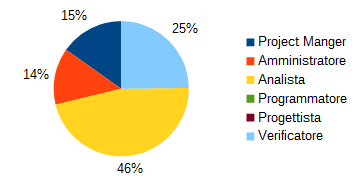
\includegraphics[width=1\linewidth]{immagini/grafici/analisi-torta.png}
		\caption{Ore per ruoli, periodo di Analisi}
	\end{figure}
	\begin{figure}[H]
		\centering
		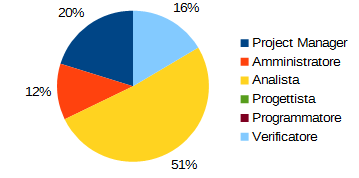
\includegraphics[width=1\linewidth]{immagini/grafici/analisi-torta-costo.png}
		\caption{Costi per ruoli, periodo di Analisi}
	\end{figure}
	\subsection{Consolidamento dei Requisiti}
	Nel periodo di \textbf{Consolidamento dei Requisiti} le ore tra i ruoli sono state divise nel seguente modo: \\
	\begin{table}[H]
		\centering
		\begin{tabular}{|c|c|c|}
			\hline
			\textbf{Ruolo}		& \textbf{Ore}	& \textbf{Costo} \\
			\hline
			Project Manager		& 1				& 30	\\
			Amministratore		& 2				& 40	\\
			Analista			& 22			& 550	\\
			Progettista			& 0				& 0	\\
			Programmatore		& 0				& 0	\\
			Verificatore		& 5				& 75	\\
			\hline
			\textbf{Totale}		& 30			& 695	\\
			\hline
		\end{tabular}
		\caption{Ore per ruolo, periodo di Consolidamento dei Requisiti}
		\end{table}
	I seguenti grafici illustrano rispettivamente come ciascun ruolo abbia influito sul totale
delle ore e dei costi del periodo di \textbf{Consolidamento dei Requisiti}. \\
	\begin{figure}[H]
		\centering
		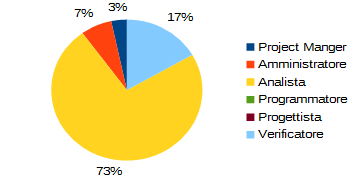
\includegraphics[width=1\linewidth]{immagini/grafici/analisi_dettaglio-torta.png}
		\caption{Ore per ruoli, periodo di Consolidamento dei Requisiti}
	\end{figure}
	\begin{figure}[H]
		\centering
		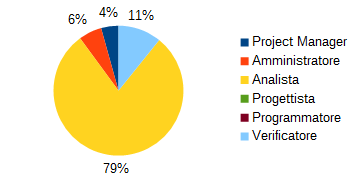
\includegraphics[width=1\linewidth]{immagini/grafici/analisi_dettaglio-torta-costo.png}
		\caption{Costi per ruoli, periodo di Consolidamento dei Requisiti}
	\end{figure}
	\subsection{Progettazione Architetturale}
	Nel periodo di \textbf{Progettazione Architetturale} le ore tra i ruoli sono state divise nel seguente modo: \\
	\begin{table}[H]
		\centering
		\begin{tabular}{|c|c|c|}
			\hline
			\textbf{Ruolo}		& \textbf{Ore}	& \textbf{Costo} \\
			\hline
			Project Manager		& 10			& 300	\\
			Amministratore		& 7				& 142	\\
			Analista			& 21			& 525	\\
			Progettista			& 89			& 1958	\\
			Programmatore		& 0				& 0	\\
			Verificatore		& 35			& 525	\\
			\hline
			\textbf{Totale}		& 162			& 3448	\\
			\hline
		\end{tabular}
		\caption{Ore per ruolo, periodo di Progettazione Architetturale}
		\end{table}
	I seguenti grafici illustrano rispettivamente come ciascun ruolo abbia influito sul totale
delle ore e dei costi del periodo di \textbf{Progettazione Architetturale}. \\
	\begin{figure}[H]
		\centering
		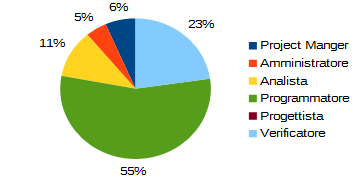
\includegraphics[width=1\linewidth]{immagini/grafici/progettazione_architetturale-torta.png}
		\caption{Ore per ruoli, periodo di Progettazione Architetturale}
	\end{figure}
	\begin{figure}[H]
		\centering
		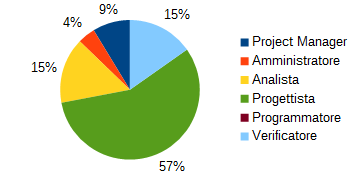
\includegraphics[width=1\linewidth]{immagini/grafici/progettazione_architetturale-torta-costo.png}
		\caption{Costi per ruoli, periodo di Progettazione Architetturale}
	\end{figure}
	\subsection{Progettazione di Dettaglio e Codifica}
	Nel periodo di \textbf{Progettazione di Dettaglio e Codifica} le ore tra i ruoli sono state divise nel seguente modo: \\
	\begin{table}[H]
		\centering
		\begin{tabular}{|c|c|c|}
			\hline
			\textbf{Ruolo}		& \textbf{Ore}	& \textbf{Costo} \\
			\hline
			Project Manager		& 10			& 300	\\
			Amministratore		& 6				& 120	\\
			Analista			& 2				& 50	\\
			Progettista			& 93			& 2046	\\
			Programmatore		& 106			& 1590	\\
			Verificatore		& 84			& 1260	\\
			\hline
			\textbf{Totale}		& 301			& 5366	\\
			\hline
		\end{tabular}
		\caption{Ore per ruolo, periodo di Progettazione di Dettaglio e Codifica}
		\end{table}
	I seguenti grafici illustrano rispettivamente come ciascun ruolo abbia influito sul totale
delle ore e dei costi del periodo di \textbf{Progettazione di Dettaglio e Codifica}. \\
	\begin{figure}[H]
		\centering
		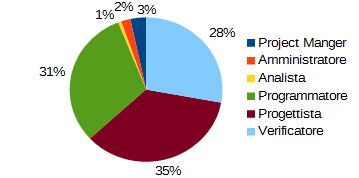
\includegraphics[width=1\linewidth]{immagini/grafici/progettazione_dettaglio_codifica-torta.png}
		\caption{Ore per ruoli, periodo di Progettazione di Dettaglio e Codifica}
	\end{figure}
	\begin{figure}[H]
		\centering
		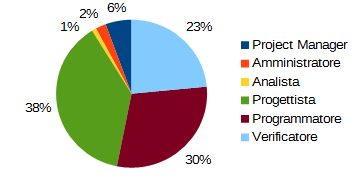
\includegraphics[width=1\linewidth]{immagini/grafici/progettazione_dettaglio_codifica-torta-costo.png}
		\caption{Costi per ruoli, periodo di Progettazione di Dettaglio e Codifica}
	\end{figure}
	\subsection{Verifica e Validazione}
	Nel periodo di \textbf{Verifica e Validazione} le ore tra i ruoli sono state divise nel seguente modo: \\
	\begin{table}[H]
		\centering
		\begin{tabular}{|c|c|c|}
			\hline
			\textbf{Ruolo}		& \textbf{Ore}	& \textbf{Costo} \\
			\hline
			Project Manager		& 11			& 330	\\
			Amministratore		& 22			& 440	\\
			Analista			& 0				& 0	\\
			Progettista			& 15			& 330	\\
			Programmatore		& 33			& 495	\\
			Verificatore		& 54			& 810	\\
			\hline
			\textbf{Totale}		& 135			& 2405	\\
			\hline
		\end{tabular}
		\caption{Ore per ruolo, periodo di Verifica e Validazione}
		\end{table}
	I seguenti grafici illustrano rispettivamente come ciascun ruolo abbia influito sul totale
delle ore e dei costi del periodo di \textbf{Verifica e Validazione}. \\
	\begin{figure}[H]
		\centering
		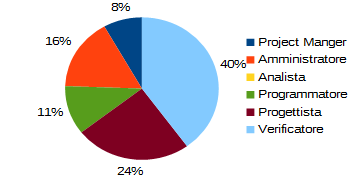
\includegraphics[width=1\linewidth]{immagini/grafici/validazione-torta.png}
		\caption{Ore per ruoli, periodo di Verifica e Validazione}
	\end{figure}
	\begin{figure}[H]
		\centering
		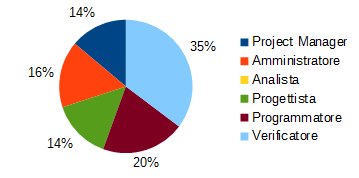
\includegraphics[width=1\linewidth]{immagini/grafici/validazione-torta-costo.png}
		\caption{Costi per ruoli, periodo di Verifica e Validazione}
	\end{figure}
	\subsection{Totale}
		\subsubsection{Ore totali con investimento}
		Le ore totali, previste per la realizzazione dell'intero progetto, comprese le ore di investimento, sono riportate nella tabella seguente. \\
		\begin{table}[H]
		\centering
		\begin{tabular}{|c|c|c|}
			\hline
			\textbf{Ruolo}		& \textbf{Ore}	& \textbf{Costo} \\
			\hline
			Project Manager		& 51			& 1530	\\
			Amministratore		& 54			& 1080	\\
			Analista			& 103			& 2575	\\
			Progettista			& 197			& 4334	\\
			Programmatore		& 139			& 2085	\\
			Verificatore		& 209			& 3135	\\
			\hline
			\textbf{Totale}		& 753			& 14739	\\
			\hline
		\end{tabular}
		\caption{Ore totali per ruolo}
		\end{table}
		I seguenti grafici illustrano rispettivamente come ciascun ruolo abbia influito sul totale delle ore e dei costi di tutto il progetto compresa la fase di investimento. \\
		\begin{figure}[H]
		\centering
			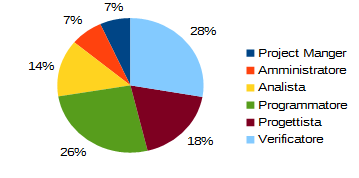
\includegraphics[width=1\linewidth]{immagini/grafici/riepilogo_conclusivo-torta.png}
			\caption{Ore totali per ruoli}
		\end{figure}
		\begin{figure}[H]
			\centering
			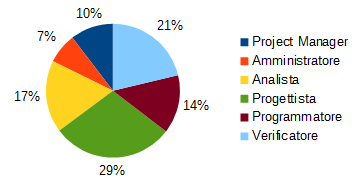
\includegraphics[width=1\linewidth]{immagini/grafici/riepilogo_conclusivo-torta-costo.png}
			\caption{Costi totali per ruoli}
		\end{figure}
		\subsubsection{Ore rendicontate}
		Le ore totali rendicontate sono riportate nella tabella sottostante, insieme al costo totale del progetto a carico del committente. \\
		\begin{table}[H]
		\centering
		\begin{tabular}{|c|c|c|}
			\hline
			\textbf{Ruolo}		& \textbf{Ore}	& \textbf{Costo} \\
			\hline
			Project Manager		& 31			& 930	\\
			Amministratore		& 35			& 700	\\
			Analista			& 23			& 575	\\
			Progettista			& 197			& 4334	\\
			Programmatore		& 139			& 2085	\\
			Verificatore		& 173			& 2595	\\
			\hline
			\textbf{Totale}		& 598			& 11219	\\
			\hline
		\end{tabular}
		\caption{Ore totali retribuite per ruolo}
		\end{table}
		I seguenti grafici illustrano rispettivamente come ciascun ruolo abbia influito sul totale delle ore e dei costi retribuiti. \\
		\begin{figure}[H]
		\centering
			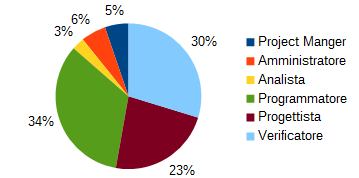
\includegraphics[width=1\linewidth]{immagini/grafici/orario_rendicontato-torta.png}
			\caption{Ore totali retribuite per ruoli}
		\end{figure}
		\begin{figure}[H]
			\centering
			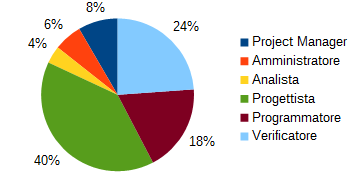
\includegraphics[width=1\linewidth]{immagini/grafici/orario_rendicontato-torta-costo.png}
			\caption{Costi totali retribuiti per ruoli}
		\end{figure}
		\subsubsection{Conclusioni}
		Il costo totale viene arrotondato a € 11250. \\
		Si è scelto di proporre un preventivo economico maggiorato rispetto a quello calcolato poiché, nonostante la sua irrisorietà, tale maggiorazione permetterà in caso di necessità di poter disporre di ore di lavoro aggiuntive senza dover incidere sui costi proposti.